\documentclass[10pt,a4paper]{report}

% localização com hifenização
\usepackage[utf8]{inputenc}
\usepackage[brazil]{babel}
\usepackage{graphicx}
\usepackage{epsfig}
\usepackage{cite}
\usepackage{textcomp} %para o greater than
\usepackage[margin=1in]{geometry}

\usepackage{enumerate}
\usepackage{xspace}
\usepackage{colortbl}
\usepackage{listings}             % Include the listings-package
\lstset{numbers=left, stepnumber=1, frame=single, rulesepcolor=\color{blue}, language=C}

\graphicspath{{./../images/}}

\begin{document}

\tableofcontents

% ------------------------------------------------------------------------------------------------
% Apresentação
% ------------------------------------------------------------------------------------------------
 
\chapter{Apresentação}

O Pure Data á um ambiente visual de programação musical que permite criarmos
aplicações musicais complexas a partir da combinação de componentes visuais.
Apesar do Pure Data conter vários componentes prontos há a possibilidade de
criarmos novos objetos em C/C++. Estes objetos são chamados de externals.

Este é um tutorial prático para escrita de externals em C para o Pure Data. A
iniciativa de escrever tal documento surgiu na disciplina de Computação
Musical do Instituto de Matemática e Estatísticas da Universidade de São Paulo
no primeiro semestre de 2011 ministrada pelo professor Marcelo Gomes de
Queiroz. A intenção deste tutorial é tentar auxiliar programadores a
desenvolver externals de maneira bastante simples.

Mais do que ampliar a gama de objetos do Pure Data e criar novos objetos, o objetivo deste trabalho é também permitir ao pesquisador de computação musical a implementação e testes de algoritmos de processamento de áudio para caráter de estudo. Isto significa que podemos reimplementar várias coisas que já existem no Pure Data simplesmente porque é didático programar e colocar algoritmos para funcionar.

\section{Escrevendo seus externals}

O Pure Data possui uma API para o desenvolvimento de externals. Para utilizar esta API é necessário importar a biblioteca m\_pd.h que está disponível em (http://compbio.cs.toronto.edu/repos/snowflock/mpich-1.2.7/mpid/mpd/mpd.h). Há um tutorial para escrever externals feito pelo IOHannes, um dos programadores do Pure Data. Este tutorial está disponível em http://iem.at/pd/externals-HOWTO/pd-externals-HOWTO.pdf. Apesar deste documento ter sido meu ponto de partida, boa parte do que contém no presente tutorial foi aprendido lendo código-fonte de externals do repositório do próprio Pure Data (http://pure-data.svn.sourceforge.net/viewvc/pure-data/trunk/externals/).

\section{Organizando seus externals}
É praxe que o arquivo do external tenha o mesmo nome que o external. Se fossemos fazer, por exemplo, um trigger, o mesmo estaria em um arquivo chamado trigger.c e seria compilado em um external chamado trigger.pd\_linux ou trigger.dll ou trigger.pd\_irix5 ou trigger.pd\_darwin. Isto não é obrigatório mas é uma convenção que facilita a busca do código-fonte deste external no repositório.

\section{Compilando seus externals}

Um external precisa ser compilado e depois linkado como external. A versão Linux pode ser feita com os comandos:

\begin{lstlisting}
cc -DPD -O2 -fPIC -funroll-loops -fomit-frame-pointer 
	-Wall -W -Wshadow -Wstrict-prototypes -Werror 
	-Wno-unused -Wno-parentheses -Wno-switch 
	-o example1.o -c example1.c
ld -export_dynamic  -shared -o example1.pd_linux 
	example1.o -lc -lm
rm example1.o
\end{lstlisting}

Para compilar, o ideal é criarmos um Makefile. Todas as pastas de exemplos deste tutorial estão acompanhadas de um makefile feito pelo Marcelo Queiroz.

\section{Criando help para seus externals}

O arquivo de help deve ter o mesmo nome que o external. Por exemplo, para o exemplo1.c com o objeto exemplo1 temos o arquivo example1-help.pd. Este arquivo do puredata com exemplo deve acompanhar o external na instalação, ficando na mesma pasta que o external compilado.
Há a possibilidade de associarmos a cada external outros arquivos que não sigam esta convenção e a mesma será apresentada no próximo capítulo.

\section{Executando seu external}

Se você executar o Pure Data na mesma pasta aonde está seu external compilado, o mesmo irá funcionar. Caso não esteja executando o pure data via terminal deverá colocar a pasta aonde o external se encontra no caminho de busca do Pure Data.
\begin{figure}[h!]
	\centering
	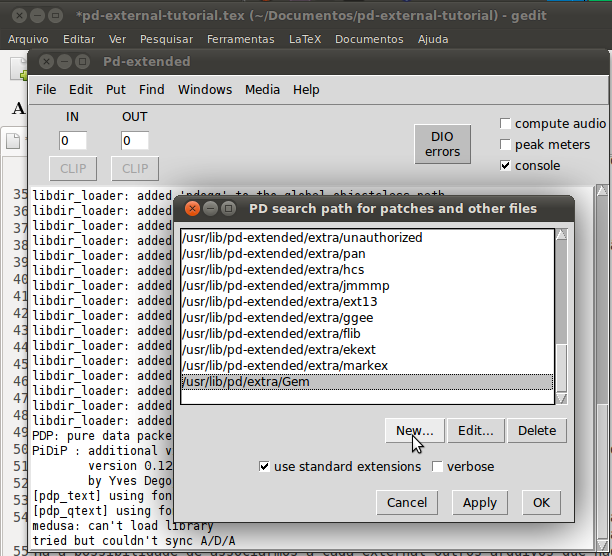
\includegraphics[width=0.7\textwidth]{path}
	\caption{Adicionando o diretório do seu external no Pure Data.}
\end{figure}

Para carregar uma biblioteca de externals (mais de um external no mesmo arquivo-fonte), é necessário adicionar a biblioteca no Pure Data:

 
\begin{lstlisting}
pdextended  -lib medusa medusa-help.pd 
\end{lstlisting}

Ou 

\begin{figure}[h!]
	\centering
	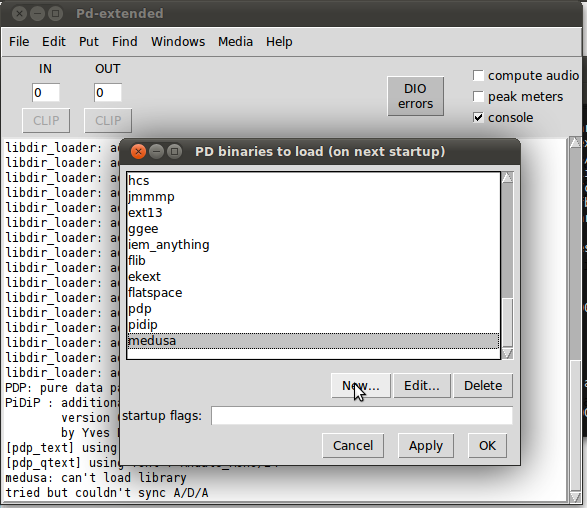
\includegraphics[width=0.7\textwidth]{startup}
	\caption{Adicionando sua biblioteca no Pure Data.}
\end{figure}

% ------------------------------------------------------------------------------------------------
% O básico de um external
% ------------------------------------------------------------------------------------------------

\chapter{O básico de um external}

Escrever um external significa seguir as recomendações da API. Peço ao leitor bastante paciência pois este tutorial pretende andar um pouco devagar para mostrar os passos da escrita de um external.

\section{Meu primeiro external}

Um external necessita de uma estrutura de dados como uma classe em C. Esta estutura deverá obrigatoriamente possuir um atributo do tipo t\_object. Outros atributos podem ser adicionados nesta estrutura de maneira que cada instância da mesma possua os dados necessários para sua execução. Um objeto contador, por exemplo, pode constar o contador e um objeto que abra um arquivo pode possuir o caminho do arquivo. O básico desta estrutura é mostrado abaixo.

\begin{lstlisting}

static t_class *example1_class;

typedef struct _example1 {
    t_object x_obj;
} t_example1;
\end{lstlisting}

Todo external deve ter um método com o nome do próprio arquivo + \_setup(). Assim, o puredata irá procurar no arquivo trigger.pd\_linux o método trigger\_setup(void) e no arquivo osc$\sim$.pd\_linux o método osc\_tilde\_setup(void). Independente de o mesmo ser um único external ou uma biblioteca. Veja que objetos que recebem áudio e que, por consequência possuem $\sim$ no seu nome, possuem \_tilde\_setup na assinatura de seu método. É do método setup() que começamos tudo.

\begin{lstlisting}

void example1_setup(void) {
    example1_class = class_new(gensym("example1"),
            (t_newmethod) example1_new, // Constructor
            0,
            sizeof (t_example1),
	    CLASS_NOINLET,
            0);
}
\end{lstlisting}

Na chamada do método setup() podemos ter a construção de um objeto (Veja o exemplo 01) ou uma biblioteca com vários objetos (Veja exemplo 03). A construção de um objeto é feita a partir da função class\_new(). Esta função recebe vários parâmetros como:
\begin{itemize}
\item nome do objeto
\item função construtora do objeto
\item função destrutora do objeto
\item tamanho do objeto
\item Tipo da classe do objeto
\item Parâmetros a serem passados para o objeto na sua construção (Podem ser vários - Veja o próximo capítulo)
\item Zero.
\end{itemize}

É obrigatório que o último parâmetro seja 0 pois isto indicará ao PD que os parâmetros terminaram.

O tipo da classe pode definir seu comportamento. Estes tipos são:

\begin{itemize}
\item CLASS\_DEFAULT 0
\item CLASS\_PD 1
\item CLASS\_GOBJ 2
\item CLASS\_PATCHABLE 3
\item CLASS\_NOINLET 8
\end{itemize}

(Retirado do arquivo m\_pd.h)

*** Usei apenas o 0 e o 8. Experimentarei usar os outros tipos.

A função class\_new() será utilizada para construir o objeto. Nesta função, além de criarmos o novo objeto com a função pd\_new, podemos definir os valores dos atributos da nossa estrutura de dados e inicializar qualquer contexto que seja necessário, como abrir arquivos, popular arrays e outras coisas.

\begin{lstlisting}
// Constructos of the class
void * example1_new(void) {
    t_example1 *x = (t_example1 *) pd_new(example1_class);
    return (void *) x;
}
\end{lstlisting}

Se tudo foi feito corretamente, compilado e colocado no PD, temos o resultado.

\begin{figure}[h!]
	\centering
	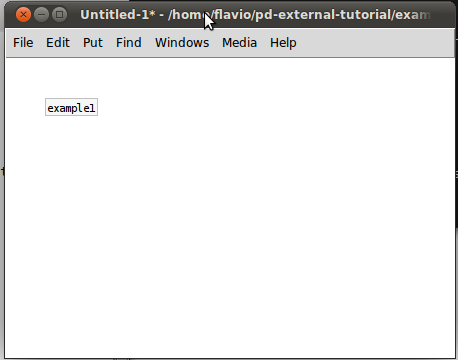
\includegraphics[width=0.7\textwidth]{example1}
	\caption{Nosso primeiro external do PD. Ainda inútil.:-)}
\end{figure}

\section{Minha primeira biblioteca}

Um mesmo método setup pode definir vários objetos de classes diferentes. A isto damos o nome de biblioteca. Para isto, o método setup() terá o mesmo nome do arquivo com a biblioteca mas os objetos podem ter outros nomes. Veja o exemplo03.

\begin{lstlisting}

void example3_setup(void) {
    post("Initializing my library");

    myobj1_class = class_new(gensym("myobj1"),
            (t_newmethod) myobj1_new, // Constructor
            0,
            sizeof (t_myobj1),
	    CLASS_NOINLET,
            0);
    class_sethelpsymbol(myobj1_class, 
	gensym("myobj1-help"));

    myobj2_class = class_new(gensym("myobj2"),
            (t_newmethod) myobj2_new, // Constructor
            0,
            sizeof (t_myobj2),
	    CLASS_NOINLET,
            0);
    class_sethelpsymbol(myobj2_class, 
	gensym("myobj2-help"));

}
\end{lstlisting}

Se o arquivo foi feito corretamente, compilado corretamente e adicionado ao caminho do PureData, teremos o resultado.

\begin{figure}[h!]
	\centering
	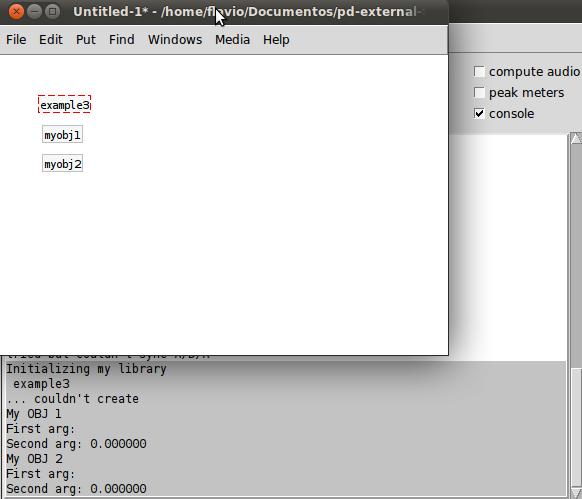
\includegraphics[width=0.7\textwidth]{example3}
	\caption{Nosso primeiro external do PD. Ainda inútil.:-)}
\end{figure}


No caso da biblioteca, podemos ter um arquivo de help para cada external. Esta associação é feita pela função:
\begin{lstlisting}
class_sethelpsymbol(myclass_class, gensym("my_class-help"));
\end{lstlisting}

Um objeto pode ainda ter outros nomes ou alias. Para definir isto podemo utilizar a função class\_addcreator. Veja o exemplo:

\begin{lstlisting}
class_addcreator((t_newmethod)medusa_new, gensym("med"), 0);
\end{lstlisting}

\section{Variáveis globais}
Você pode usar uma variável global para armazenar dados pelos seus externals. Esta variável será visível para todas as intâncias do external e todas podem alterar seu valor. Isto pode ser útil ou um desastre. (Veja o exemplo16).

\begin{lstlisting}
int count = 0;

void * example16_new(void) {
    t_example16 *x = (t_example16 *) pd_new(example16_class);
    post("Counter value: %d",count);
    count++;
    return (void *) x;
}
\end{lstlisting}

\begin{figure}[h!]
	\centering
	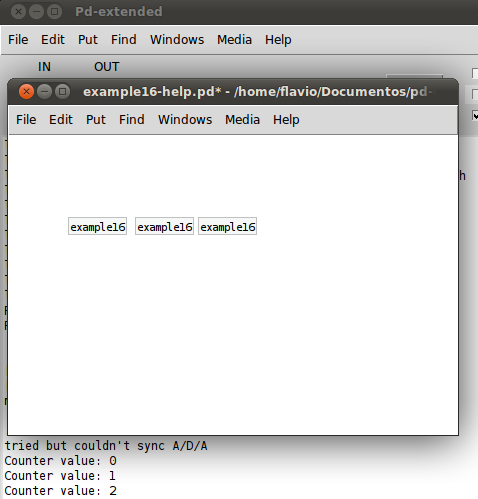
\includegraphics[width=0.7\textwidth]{example16}
	\caption{Repare no output da janela principal.}
\end{figure}

Caso isto não seja desejável, o ideal é colocar suas variáveis dentro da struct do objeto. Assim cada instância terá seu próprio contador.

\begin{lstlisting}

static t_class *example_class;

typedef struct _example {
    t_object x_obj;
    t_int counter;
} t_example;

void * example_new(void) {
    t_example *x = (t_example *) pd_new(example_class);
    post("Counter value: %d",x->counter);
    counter++;
    return (void *) x;
}

\end{lstlisting}

% ------------------------------------------------------------------------------------------------
% OS TIPOS DE DADOS DO PD
% ------------------------------------------------------------------------------------------------

\chapter{Os tipos de dados do PD}

Você pode usar os tipos de dados padrões do C, como int, float ou char. O difícil é entender o que chamamos de tipos de dados padrões do C já que estes tipos podem variar de acordo com o sistema operacional, compilador e outras coisas. Por isto, para o external possa se comportar da mesma maneira em qualquer sistema, é bastante recomendado que usemos os tipos do pure data.

Os tipos do pure data nada mais são que um

% ------------------------------------------------------------------------------------------------
% CONSTRUTOR E DESTRUTOR
% ------------------------------------------------------------------------------------------------

\chapter{Construtor e destrutor}

O Construtor de um objeto pode receber parâmetros. Estes parâmetros são ilustrados abaixo.

\begin{figure}[h!]
	\centering
	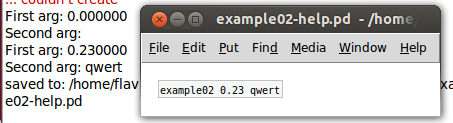
\includegraphics[width=0.7\textwidth]{example2}
	\caption{External recebendo parâmetros. Note a tela de saída no fundo da imagem.}
\end{figure}

\section{Construtor}

Parâmetros de inicialização no construtor podem permitir que inicializemos o external com determinados valores. Isto é feito definindo os parâmetros no métodos class\_new() quanto na definição da função construtora. (Veja o exemplo02).

\begin{lstlisting}

// Constructos of the class
void * example2_new(t_symbol * arg1, t_floatarg arg2) {
    t_example2 *x = (t_example2 *) pd_new(example2_class);
    post("First arg: %s", arg1->s_name);
    post("Second arg: %f", arg2);
    return (void *) x;
}

void example2_setup(void) {
    example2_class = class_new(gensym("example2"),
            (t_newmethod) example2_new, // Constructor
            0,
            sizeof (t_example2),
	    CLASS_NOINLET,
            A_DEFFLOAT, // First Constructor parameter
            A_DEFSYMBOL, // Second Consctructo parameter
            0);
}
\end{lstlisting}

Notem que os parâmetros são definidos com um tipo e são recebidos com outro. São tipos padrões do Pure Data. Estes tipos são chamados atom e alguns estão documentados no tutorial do IOHannes. Eles são:
\begin{itemize}
\item A\_NULL,
\item A\_FLOAT,
\item A\_SYMBOL,
\item A\_POINTER,
\item A\_SEMI,
\item A\_COMMA,
\item A\_DEFFLOAT,
\item A\_DEFSYM,
\item A\_DOLLAR, 
\item A\_DOLLSYM,
\item A\_GIMME,
\item A\_CANT
\end{itemize}
(Retirado do arquivo m\_pd.h)

*** Nunca usei todos eles. Pra que será que servem?

Entre estes tipos, um deles pode aceitar qualquer quantidade e tipo de parâmetros. É o A\_GIMME. (Veja o exemplo09). 

\begin{lstlisting}

// Constructos of the class
void * example9_new(t_symbol *s, int argc, t_atom * argv) {
    t_example9 *x = (t_example9 *) pd_new(example9_class);
    post("%d parameters received",argc);
    return (void *) x;
}


void example9_setup(void) {
    example9_class = class_new(gensym("example9"),
            (t_newmethod) example9_new, // Constructor
            (t_method) example9_destroy, // Destructor
            sizeof (t_example9),
	    CLASS_NOINLET,
	    A_GIMME, // Allows various parameters
            0); // LAST argument is ALWAYS zero
}
\end{lstlisting}

Quando utilizamos o A\_GIMME a função construtora trabalha como um programa main em C. Recebe os parâmetros argv e argc, um com uma lista de atoms e outro com a quantidade de atoms nesta lista.

\begin{figure}[h!]
	\centering
	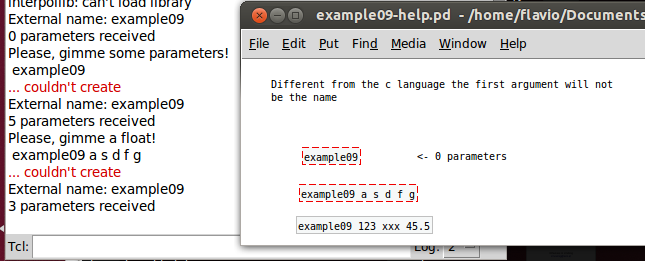
\includegraphics[width=0.7\textwidth]{example9}
	\caption{Diferente da linguagem C, o primeiro parâmetro não é o nome do external.}
\end{figure}

Note que o Pure Data não obriga que o usuário passe parâmetros para o objeto. É como se todo construtor, independentemente de como ele está definido, aceitasse sua instanciação vazia. Cabe ao programador verificar se os parâmetros recebidos são em quantidade, tipo e valor esperado e, caso não seja, abortar a construção do objeto e não retornar sua instância.

\section{Destrutor}
O destrutor de uma classe permite liberar a memória do Pure Data dos dados que foram alocados. (Veja o exemplo07)
\begin{lstlisting}
// Destroy the class
void example9_destroy(t_example9 *x) {
   post("You say good bye and I say hello");
}

void example9_setup(void) {
    example9_class = class_new(gensym("example9"),
            (t_newmethod) example9_new, // Constructor
            (t_method) example9_destroy, // Destructor
            sizeof (t_example9),
	    CLASS_NOINLET,
	    A_GIMME, // Allows various parameters
            0); // LAST argument is ALWAYS zero
}

\end{lstlisting}

A liberação da memória pode ser feita com a função freebytes() definida na API do Pure Data.

\begin{lstlisting}
void freebytes(void *x, size_t nbytes)
\end{lstlisting}

% ------------------------------------------------------------------------------------------------
% INLETS E OUTLETS
% ------------------------------------------------------------------------------------------------

\chapter{Inlets e outlets}
Os objetos que criamos até agora são inúteis. Não servem para nada. Para serem mais úteis precisamos permitir que os mesmos se comuniquem com outros objetos do Pure Data. Isto é feito por meio de Inlets e outlets. Temos dois tipos de inlets: passivos e ativos. 

\section{Inlets passivos}
Inlets passivos são inlets cuja entrada é associada a um atributo do objeto. São chamados de passivos pois a alteração do seu valor não irá iniciar a execução de uma função. Já os inlets ativos são associados a funções e permitem um pouco mais de ação quando um valor é atribuído.

\begin{lstlisting}
static t_class *example4_class;

typedef struct _example4 {
    t_object x_obj;
    t_float my_float;// Creates a my_float variable into the structure
} t_example4;


// Constructos of the class
void * example4_new(t_symbol * arg1, t_floatarg arg2) {
    t_example4 *x = (t_example4 *) pd_new(example4_class);
    post("First arg: %s", arg1->s_name);
    post("Second arg: %f", arg2);

    floatinlet_new(&x->x_obj, &x->my_float); //create a passive inlet which value will be stored into my_float variable

    return (void *) x;
}
\end{lstlisting}

O inlet passivo depende que a variável que irá armazenar o valor seja do mesmo tipo que a função usada para a criação do inlet (Veja o exemplo04). Os tipos de inlets passivos são:

\begin{itemize}
\item floatinlet\_new(t\_object *owner, t\_float *fp)
\item symbolinlet\_new(t\_object *owner, t\_symbol **sp)
\item pointerinlet\_new(t\_object *owner, t\_gpointer *gp)
\end{itemize}

\begin{figure}[h!]
	\centering
	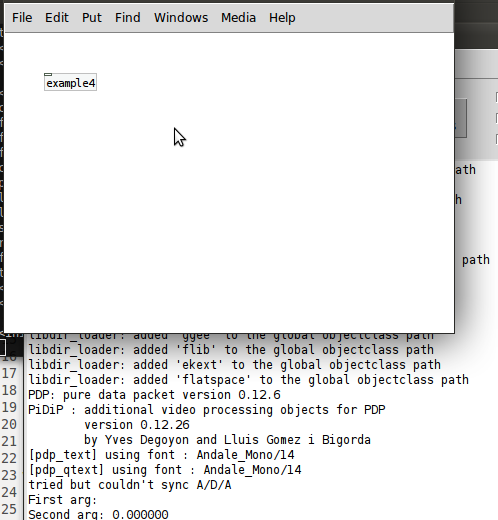
\includegraphics[width=0.7\textwidth]{example4}
	\caption{Inlets passivos}
\end{figure}

\section{Inlets ativo}
Um inlet ativo associa ao inlet uma função. Assim como o inlet passivo, a criação de um inlet ativo permite definir o tipo do dado que o inlet irá receber.(Veja o exemplo05).

\begin{lstlisting}
// The method will always receive the class as argument
void example5_bang(t_example5 *x) { 
    post("BANGED!");
    post("My_float value: %f",x->my_float);
}

void example5_anything(t_example5 *x, t_symbol *s, int argc, t_atom *argv){
	post("ANYTHING!");
}

void example5_setup(void) {
    example5_class = class_new(gensym("example5"),
            (t_newmethod) example5_new, // Constructor
            0, 
            sizeof (t_example5),
	    CLASS_DEFAULT,
            0); // LAST argument is ALWAYS zero
    class_addbang(example5_class, example5_bang);
    class_addanything(example5_class, example5_anything);
}
\end{lstlisting}

Este é o resultado:

\begin{figure}[h!]
	\centering
	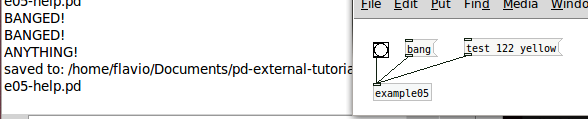
\includegraphics[width=0.7\textwidth]{example5}
	\caption{Inlets.}
\end{figure}

Os tipos definidos na criação de inlets dependem da função que irá receber o conteúdo deste inlet possuir a assinatura correta. São elas:

\begin{table}[ht]
\centering
\begin{tabular}{ll}
\hline
\hline
void class\_addbang(t\_class *c, t\_method fn); 	& void my\_bang\_method(t\_mydata *x); \\
void class\_addfloat(t\_class *c, t\_method fn);	& void my\_float\_method(t\_mydata *x, t\_floatarg f); \\
void class\_addsymbol(t\_class *c, t\_method fn);	& void my\_symbol\_method(t\_mydata *x,t\_symbol *s); \\
void class\_addpointer(t\_class *c, t\_method fn);	& void my\_pointer\_method(t\_mydata *x, t\_gpointer *pt); \\
void class\_addlist(t\_class *c, t\_method fn);		& void my\_list\_method(t\_mydata *x, t\_symbol *s, int argc, t\_atom *argv); \\
void class\_addanything(t\_class *c, t\_method fn);	& void my\_any\_method(t\_mydata *x, t\_symbol *s, int argc, t\_atom *argv); \\
\hline
\hline
\end{tabular}
\end{table}

\section{Um inlet com várias mensagens}

Um inlet pode ainda receber vários tipos de mensagens diferentes e associar métodos diferentes para tratar cada tipo de mensagem. Isto é feito com a função add\_method.  (Veja o exemplo08).

\begin{lstlisting}
// Constructos of the class
void * example8_new(void) {
    t_example8 *x = (t_example8 *) pd_new(example8_class);

    // creating inlets to the messages "alfa"
    inlet_new(&x->x_obj, &x->x_obj.ob_pd, gensym("float"), gensym("alfa"));

    return (void *) x;
}

void example8_start(t_example8 *x){
    post("START / BANG");
}

void example8_open(t_example8 *x, t_symbol *s){
    post("open %s",s->s_name);
}


void example8_alfa(t_example8 *x, t_floatarg f){
	post("ALFA VALUE %f",f);
}

void example8_setup(void) {
    example8_class = class_new(gensym("example8"),
            (t_newmethod) example8_new, // Constructor
            (t_method) example8_destroy, // Destructor
            sizeof (t_example8),
	    CLASS_DEFAULT,
            0); // LAST argument is ALWAYS zero

    // All these messages will be received by the first left inlet
    class_addmethod(example8_class, (t_method) example8_start, 
	gensym("start"), 0); // two messages, the same function
    class_addmethod(example8_class, (t_method) example8_start, 
	gensym("bang"),  0); // may be "start" or "bang" messages
    class_addmethod(example8_class, (t_method) example8_open,  
	gensym("open"),  A_DEFSYMBOL,0);

    // These messages will be associated with inlet 2
    class_addmethod(example8_class, (t_method) example8_alfa,  
	gensym("alfa"), A_DEFFLOAT,0); 

}
\end{lstlisting}

Desta forma não precisamos tratar a mensagem que o inlet recebe mas definí-las de antemão e criar funções que mapeiem a mensagem recebida.

\begin{figure}[h!]
	\centering
	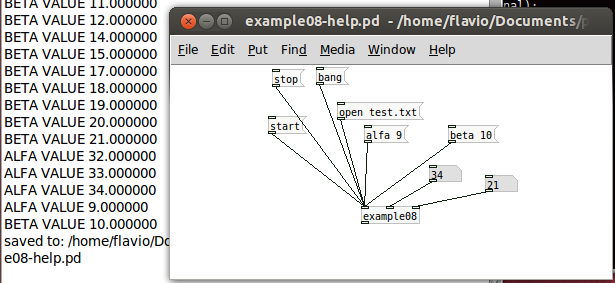
\includegraphics[width=0.7\textwidth]{example8}
	\caption{Mais inlets.}
\end{figure}


Note que este código possui duas abordagens para esta estrutura de inlets. Uma é associar o tipo da mensagem e o parâmetro a um método e outra é criar um inlet "genérico" que vai associar a mensagem a um novo inlet. Isto é feito pela função inlet\_new.

\begin{lstlisting}
t_inlet *inlet_new(t_object *owner, t_pd *dest,
      t_symbol *s1, t_symbol *s2);
\end{lstlisting}

\section{Oulets}

Depois de termos tratados as formas de entrada de dados para o inlet do PD, chegou a hora de tratarmos as saídas. Isto é feito por meio de outlets. (Veja o exemplo06).

\begin{lstlisting}

typedef struct _example6 {
    t_object x_obj;
    t_outlet *my_outlet; // Defines an outlet
} t_example6;

// The BANG method, first inlet

void example6_bang(t_example6 *x) {
    post("BANGED!");
    outlet_bang(x->my_outlet); // Bang my outlet
}

// Constructos of the class
void * example6_new(t_symbol * arg1, t_floatarg arg2) {
    t_example6 *x = (t_example6 *) pd_new(example6_class);

    x->my_outlet = outlet_new(&x->x_obj, gensym("bang"));

    return (void *) x;
}

void example6_setup(void) {
    example6_class = class_new(gensym("example6"),
            (t_newmethod) example6_new, // Constructor
            0, 
            sizeof (t_example6),
	    CLASS_DEFAULT,
            A_DEFFLOAT, // First Constructor parameter
            A_DEFSYMBOL, // Second Consctructo parameter
            0); // LAST argument is ALWAYS zero
    class_addbang(example6_class, example6_bang);
}
\end{lstlisting}

Um outlet deve ser definido na estrutura do objeto e instanciado pela função outlet\_new. Isto permite também definirmos o tipo de dado que ele terá. No caso deste exemplo, o outlet possui um bang e disparará o bang toda vez que receber um bang.

\begin{figure}[h!]
	\centering
	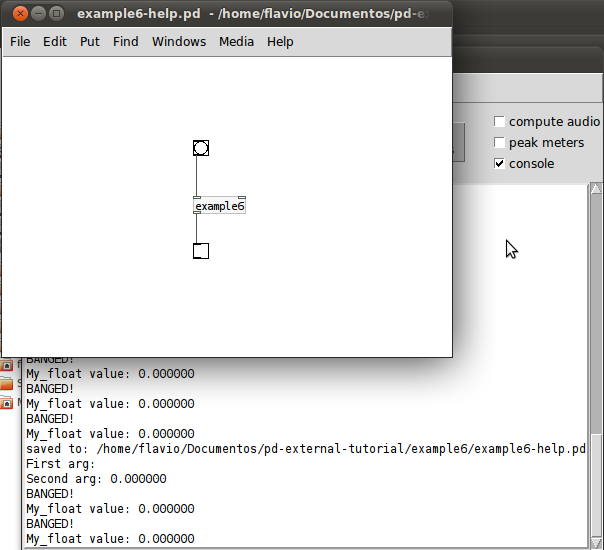
\includegraphics[width=0.7\textwidth]{example6}
	\caption{Um external bem útil que recebe um bang e envia um bang.}
\end{figure}


*** What about the proxy active inlets? It allows to define on the fly the number of inlets in a object.

% ------------------------------------------------------------------------------------------------
% DSP
% ------------------------------------------------------------------------------------------------

\chapter{DSP}
 (Precisa mudar o nome dos exemplos para exemplo~. Neste caso, a função setup deve ser renomeada para "tilde\_setup")

Enfim chegamos no processamento de áudio propriamente dito. Digital Signal Processing ou processamento de sinal digital. O PD tem inlets especiais para o processamento de sinal. É fácil reconhecer. Eles são pintados de preto.
\begin{figure}[h!]
	\centering
	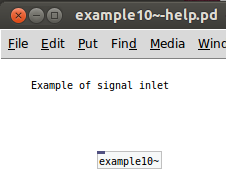
\includegraphics[width=0.7\textwidth]{example10}
	\caption{Primeiro Inlet DSP}
\end{figure}

\section{Primeiro inlet para DSP}
Para trabalharmos com DSP no Pure Data é necessário alguns cuidados. (Veja o exemplo10) Primeiramente, temos de ter na estrutura de dados um atributo do tipo t\_float para armazenar o valor de entrada do inlet.

\begin{lstlisting}
typedef struct _example10 {
    t_object x_obj;
    t_float x_f;
/* place to hold inlet's value if it's set by message */
} t_example10;
\end{lstlisting}

Caso trabalhemos com apenas um inlet de DSP, o mesmo pode utilizar o atributo "mágico" do primeiro inlet da esquerda. Isto pode ser feito com a atribuição do atributo ao inlet DSP no método setup(). Para isto temos de utilizar o tipo de classe padrão do Pure Data (CLASS\_DEFAULT). Também é necessário definirmos qual será o método chamado quando o DSP é iniciado. Este método é adicionado como os métodos dos inlets vistos anteriormente tendo porém sua mensagem associada ao tipo "dsp".

\begin{lstlisting}
void example10_setup(void) {
    example10_class = class_new(gensym("example10"),
            (t_newmethod) example10_new, // Constructor
            (t_method) example10_destroy, // Destructor
            sizeof (t_example10),
	    CLASS_DEFAULT,
	    A_GIMME, // Allows various parameters
            0); // LAST argument is ALWAYS zero

  /* this is magic to declare that the leftmost, "main" inlet
     takes signals; other signal inlets are done differently...*/
     CLASS_MAINSIGNALIN(example10_class, t_example10, x_f);

   // This method will add a signal inlet and associate a method to do this
    class_addmethod(example10_class, (t_method) example10_dsp, 
	gensym("dsp"), 0); 

}
\end{lstlisting}
 
A declaração de outros inlets DSP será vista logo adiante.

O próximo passo é definirmos o método DSP definido no setup().

\begin{lstlisting}
static void example10_dsp(t_example10 *x, t_signal **sp){
  dsp_add(example10_perform, 3, sp[0]->s_vec, sp[0]->s_n, x); 
}
\end{lstlisting}

O método associado ao DSP será chamado TODA VEZ QUE O DSP FOR INICIADO. Por isto, cuidado com alocações de memória, inicialização de variáveis e estas coisas. Neste método definiremos quem será chamado em cada laço de execução de processamento de áudio do PD. Neste cado é a função example10\_perform. Este método recebe o array de sinal que a conexão deste inlet traz. Este sinal está na variável **sp. Na atribuição acima, passamos para o método perform os atributos:

\begin{itemize}
\item método perform
\item quantidade de atributos do método
\item vetor de saída
\item tamanho do vetor (tamanho do bloco)
\item instância do nosso external
\end{itemize}

Podemos passar para o método perform quaisquer parâmetros em qualquer ordem. Só é importante e óbvio que devemos lembrar quais parâmetros foram passados e em qual ordem. O próximo passo é criar o método perform propriamente dito.

\begin{lstlisting}
static t_int * example10_perform(t_int *w){
   t_float *in = (t_float *)(w[1]);
   int n = (int)(w[2]);
   t_example10 *x = (t_example10 *)(w[3]);

  //(... DO SOMETHING)

  return (w + 4); // proximo bloco
}
\end{lstlisting}

O método perform receberá como parâmetro um array com os dados que definimos no método anterior. Neste caso na posição 0 algo que eu não sei o que é, na posição 1 o vetor de saída, na posição 2 o tamanho do vetor de saída e na posição 3 a nossa estrutura de dados. Este método deve retornar a próxima posição do vetor, ou seja, o atributo de entrada + quantidade de atributos do método + 1.

\section{Vários Inlets DSP}
Podemos ter vários inlets de DSP no nosso external (Veja o exemplo 11). A criação de inlets adicionais não é feita no método setup() mas sim no construtor. Só será necessário criar o primeiro inlet se a classe não for do tipo CLASS\_DEFAULT.

\begin{lstlisting}
// Constructos of the class
void * example11_new(t_symbol *s, int argc, t_atom * argv) {
    t_example11 *x = (t_example11 *) pd_new(example11_class);
    inlet_new(&x->x_obj, &x->x_obj.ob_pd, &s_signal, &s_signal); // second
    inlet_new(&x->x_obj, &x->x_obj.ob_pd, &s_signal, &s_signal); // third
    inlet_new(&x->x_obj, &x->x_obj.ob_pd, &s_signal, &s_signal); // fourth
    return (void *) x;
}
\end{lstlisting}

Nosso método class\_addmethod é exatamente igual ao anterior mas temos uma mudança na quantidade de parâmetros por causa da quantidade de inlets.

\begin{lstlisting}
static void example11_dsp(t_example11 *x, t_signal **sp){
  dsp_add(example11_perform, 6, sp[0]->s_vec, sp[0]->s_n, x);
}
\end{lstlisting}

Note que precisamos agora alterar a quantidade de parâmetros passadas ao método perform. O método perform ficará assim:
\begin{lstlisting}
static t_int * example11_perform(t_int *w){
   t_float *in1 = (t_float *)(w[1]);
   t_float *in2 = (t_float *)(w[2]);
   t_float *in3 = (t_float *)(w[3]);
   t_float *in4 = (t_float *)(w[4]);
   int n = (int)(w[5]);
   t_example11 *x = (t_example11 *)(w[6]);
   // DO SOMETHING...
  return (w + 7); // proximo bloco
}
\end{lstlisting}

Nosso external pronto deverá ter a seguinte aparência:
\begin{figure}[h!]
	\centering
	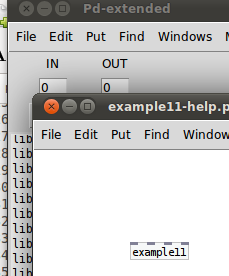
\includegraphics[width=0.7\textwidth]{example11}
	\caption{Vários inlets DSP.}
\end{figure}

\section{Primeiro outlet DSP}

A criação dos outlets é feita no construtor do external (Veja o exemplo12) e não é necessário termos adicionado os outlets a estrutura da classe.

\begin{lstlisting}
// Constructos of the class
void * example12_new(t_symbol *s, int argc, t_atom * argv) {
    t_example12 *x = (t_example12 *) pd_new(example12_class);
    outlet_new(&x->x_obj, &s_signal); // first signal outlet
    outlet_new(&x->x_obj, &s_signal); // second signal outlet
    outlet_new(&x->x_obj, &s_signal); // third signal outlet
    outlet_new(&x->x_obj, &s_signal); // fourth signal outlet
    return (void *) x;
}
\end{lstlisting}

Sabendo que temos 4 outlets, a definição do nosso método perform será idêntica ao da criação de 4 inlets.

\begin{lstlisting}
static void example12_dsp(t_example12 *x, t_signal **sp){
  dsp_add(example12_perform, 6, sp[0]->s_vec, sp[0]->s_n, x);
}
\end{lstlisting}

O método perform também será idêntico ao do exemplo com 4 inlets, porém o mesmo receberá 4 outlets.

\begin{lstlisting}
static t_int * example12_perform(t_int *w){
   t_float *out1 = (t_float *)(w[1]);
   t_float *out2 = (t_float *)(w[2]);
   t_float *out3 = (t_float *)(w[3]);
   t_float *out4 = (t_float *)(w[4]);
   int n = (int)(w[5]);
   t_example12 *x = (t_example12 *)(w[6]);
  // DO SOMETHING
  return (w + 7); // proximo bloco
}
\end{lstlisting}

\begin{figure}[h!]
	\centering
	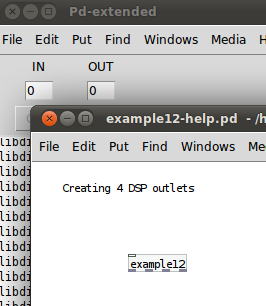
\includegraphics[width=0.7\textwidth]{example12}
	\caption{Primeiro Outlet DSP.}
\end{figure}

\section{Inlets e outlets DSP}
Nosso próximo exemplo (Veja o exemplo 13) mistura no mesmo objeto inlets e outlets DSP. Uma coisa bastante comum. Acredito que seja óbvio a construção do mesmo. Não precisamos associar estes inlets e outlets a nossa estrutura de dados. Precisamos apenas criar os inlets e outlets no construtor (lembre-se que o primeiro inlet já foi criado no método setup. Ele é mágico!).

\begin{lstlisting}
static t_int * example13_perform(t_int *w){
   t_float *in1 = (t_float *)(w[1]);
   t_float *in2 = (t_float *)(w[2]);
   t_float *in3 = (t_float *)(w[3]);
   t_float *in4 = (t_float *)(w[4]);
   t_float *out1 = (t_float *)(w[5]);
   t_float *out2 = (t_float *)(w[6]);
   t_float *out3 = (t_float *)(w[7]);
   t_float *out4 = (t_float *)(w[8]);
   int n = (int)(w[9]);
   t_example13 *x = (t_example13 *)(w[10]);
  return (w + 11); // proximo bloco
}
\end{lstlisting}

No método seguinte avisamos o método perform do tamanho dos dados.
\begin{lstlisting}
static void example13_dsp(t_example13 *x, t_signal **sp){
  dsp_add(example13_perform, 10, sp[0]->s_vec, sp[0]->s_n, x);
}
\end{lstlisting}

No método perform teremos primeiro os buffers de entrada e depois os buffers de saída.

\begin{lstlisting}
static t_int * example13_perform(t_int *w){
   t_float *in1 = (t_float *)(w[1]);
   t_float *in2 = (t_float *)(w[2]);
   t_float *in3 = (t_float *)(w[3]);
   t_float *in4 = (t_float *)(w[4]);
   t_float *out1 = (t_float *)(w[5]);
   t_float *out2 = (t_float *)(w[6]);
   t_float *out3 = (t_float *)(w[7]);
   t_float *out4 = (t_float *)(w[8]);
   int n = (int)(w[9]);
   t_example13 *x = (t_example13 *)(w[10]);
   //DO IT!
  return (w + 11); // proximo bloco
}
\end{lstlisting}

\begin{figure}[h!]
	\centering
	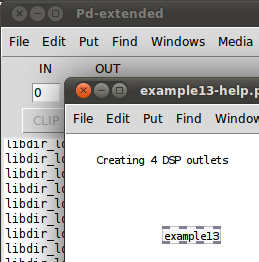
\includegraphics[width=0.7\textwidth]{example13}
	\caption{Vários inlets e outlets DSP.}
\end{figure}

\section{Inlets e outlets DSP criados dinamicamente}

Podemos definir um parâmetro no construtor que nos diga a quantidade de inlets e/ou de outlets DSP que um external terá. Neste caso, temos algumas possibilidades. A primeira é usarmos uma variável para dizer quantos inlets e outlets teremos na função dsp.

Exemplo 17

A segunda é usar outro método. Exemplo 18 - abordagem da medusa.

% ------------------------------------------------------------------------------------------------
% MULTITHREADING
% ------------------------------------------------------------------------------------------------

\chapter{Multithreading}

% ------------------------------------------------------------------------------------------------
% GUI
% ------------------------------------------------------------------------------------------------

\chapter{Externals com GUI - Usando o Tk/Tcl}
External GUIs - Using Tk/Tcl (Look the tk folder)
--------------------------------------------------------------------------
Example 14 - My First external with GUI
\begin{figure}[h!]
	\centering
	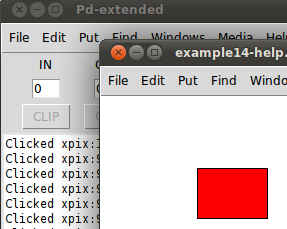
\includegraphics[width=0.7\textwidth]{example14}
	\caption{Adicionando GUI tk.}
\end{figure}

Example 15 - Adding GUI components

% ------------------------------------------------------------------------------------------------
% MISCELÂNEAS
% ------------------------------------------------------------------------------------------------

\chapter{Miscelâneas}
Como saber se um objeto existe?
pd\_findbyclass

Exemplo: http://pure-data.svn.sourceforge.net/viewvc/pure-data/trunk/pd/src/d\_array.c?revision=10432\&view=markup 

Linha 82


post

error

\end{document}

